%!TEX root = ../Thesis.tex

% 3. Method section
% In a scholarly research article, the section dealing with method is very important. The same applies to an empirical thesis. For students, this can be a difficult section to write, especially since its purpose may not always be clear.

% The method chapter should not iterate the contents of methodology handbooks. For example, if you have carried out interviews, you do not need to list all the different types of research interview. You also do not need to describe the differences between quantitative and qualitative methods, or list all different kinds of validity and reliability.

% What you must do is to show how your choice of design and research method is suited to answering your research question(s). Demonstrate that you have given due consideration to the validity and reliability of your chosen method. By “showing” instead of “telling”, you demonstrate that you have understood the practical meaning of these concepts. This way, the method section is not only able to tie the different parts of your thesis together, it also becomes interesting to read!

% Show the reader what you have done in your study, and explain why. How did you collect the data? Which options became available through your chosen approach?
% What were your working conditions? What considerations did you have to balance?
% Tell the reader what you did to increase the validity of your research. E.g., what can you say about the reliability in data collection? How do you know that you have actually investigated what you intended to investigate? What conclusions can be drawn on this basis? Which conclusions are certain and which are more tentative? Can your results be applied in other areas? Can you generalise? If so, why? If not, why not?
% You should aim to describe weaknesses as well as strengths. An excellent thesis distinguishes itself by defending – and at the same time criticising – the choices made.

\chapter{Method}
As previously mentioned the main control unit has be deployed on cRIO9033 - National Intruments' controller equipped with real-time processor and re-configurable FPGA unit. The reasoning for usage of this device was that it has more than sufficient computation power for the task and with additional modules provides support for basic CAN communication as well as high level CANOpen abstraction.


In my setup I have been using module NI9853 to directly receive and send a CAN messages and NI9881 for communication with the motor controllers based on CANOpen standard.

\section{Master control unit software implementation}
From the early beginning I have been developing the code of master control unit using event based programming paradigm. The reasoning of this is asynchronous, real-time nature of of such unit.

Most simple classification of subsystems can be based on communication protocol being used. 

\subsection{CAN integration}
To start with I had to implement a CAN library so it would be possible to make certain threads wait for message with predefined id, one from array of ids or just any message. 

To achieve it, I have a functionality deployed on FPGA (Field Programmable Gate Array) which simply translates input/output messages into the arrays of 8x unsigned integers. Read messages  are furthermore pushed into the FIFO register and interrupt on real-time processor is called.

Upon initiation of real-time programme additional process is spawned in the background which is responsible for communication with the FPGA. For sending a message it simply pushes data to FPGA and marks it as ready to send. When it comes to reading the process waits for interrupt from FPGA and acknowledges it after data read is finished. 

Then look up table is check for existence of conditional variable for given id, it is created if does not exist, and updated with new message. Additionally conditional variable containing id of last received message id is updated.

Based to this architecture I implemented functions which can wait for any message, one with certain id or one from ids set.

\subsection{Device operation states}
Although, during operation everything is event based the whole application itself can be considered a state machine where normal operation is just one of the states.

\todo{fig Init->boot-up seq->operational->exit}

\subsection{Operational state}
Implemented controller provides following functionality:
\begin{itemize}
    \item Log pedals, motor, pumps status and all occurred errors
    \item Updates motors target torque based on calculated electronic differential state (torque vectoring), power limitation and acceleration pedal position
    \item Control pumps power based on motors temperature and current target torque
    \item Subsystems connection loss procedures
    \item (Emergency) shutdown
    \item Read pedals, BMS, LV BMS and motors status.
\end{itemize}


\chapter{Overview of experimental setup}
Having not sufficient financial support enforced many compromises on design which I did not have direct influence on. The decision was made that will be running in low voltage - high current setup so we could use cost efficient lithium-ion batteries. 
Although theoretically possible cabling and connector sizing was a bit overwhelming for responsible teams.

In our final setup we used:
\begin{itemize}
    \item Two EMRAX228 motors which nominal power of about 50kW (when liquid cooled)
    \item Two emDrive500 controllers capable full usage of AM motors
    \item Arduinos with CAN shields to act as intelligent sensors/controllers
    \item Two \todo{which pump?} pumps for cooling purposes
    \item National Instruments' cRIO 9033 as a main control unit
\end{itemize}

This result in system which in simplified manner has been presented in figure \todo{figure ref}.

\todo{figure}

As shown all the communication with master control unit is based on CAN bus. 






All small subsystems are based on Arduino evaluation boards.


\subsection{Pedals sensor}
System to measure pedals and steering wheel position is based on Arduino evaluation board. Which is a simple evaluation setup build upon Atmel ATmega8 with $16MHz$ oscillator.

Now considering the sampling rate of this sub-module it has been programmed to use prescaler for A/D converter with value of 128. Referring to datasheet basic conversion takes 13 clock cycles so we should except sampling rate of about $16MHz/128/13 = 9615Hz = 104µs$ \cite{Atmega8}.

However, in electric car there is a lot of electromagnetic noise which needs to be addressed. To reduce impact of noise which was significant in first approach, code was modified to calculate average of 10 successive samples efficiently reducing sampling rate to $1,04ms$.

Considering the fact that ATmega8 consist of just one analogue-decimal converter with multiplexed input the measurement takes approximately $1,04ms * number of sensors$ \cite{Atmega8}.
To satisfy the safety requirements we needed to use two offset sensors for each pedal (accelerator, brake) and one for steering wheel. In consequence each measurement takes at least $1,04ms * 5 = 5,2ms$.

This system sense all the information which is:
\begin{itemize}
    \item pedals position
    \item steering wheel position
    \item pedals sensors position miss-match
    \item pedals, steering wheel over-travel, under-travel and connection loss errors
\end{itemize}

After the measurement the information is sent through CAN bus with baud rate of 500kbit/s (used CAN module was not capable to work with higher baud rates). Pedals position although being read on 10 bits is averaged and only 8 significant bits are sent. We assumed that 256 quantization steps is enough in this case. It allowed us shorten CAN frame to consist only 4 bytes of data.
Now considering timing, the CAN frame (\todo{CAN frame graphic (wiki like)}) consist of 44 basic bits plus 4 bytes of data in our case. The total time of sending/receiving would be therefore $\frac{76}{500kbit/s} = 152us$.

Assuming no further improvements we should expect the pedals sub-systems is capable of sending the pedals, steering wheel position in time interval of about $5,2ms$ in normal operation.
Additionally, if any of the above mentioned errors occurred the second CAN frame is sent containing two bytes with bitwise encoded errors extending the expected interval into $~5,3ms$.

\subsection{Pump control}
In our car we have used \todo{which pump} pumps, which can be controlled by signal from $0-5V$. Since used Arduino has no dedicated analogue input we made one by using the PWM signal with low-pass filter (direct control by PWM signal was strongly disapproved by the pump manufacturer \todo{cite pump manual}).
The subsystem acts simply by controlling pulse width based on the value received by CAN message from master control unit. It also provide basic emergency behaviour in the manner that if no message was sensed over one second the pumps are turned on to work with full power.






\section{Implementation of electrical differential based on steering angle}
In my implementation I have enriched calculations explained in \ref{diff_calc}. Starting with the steering wheel, the sensor output in normalised to the measured minimum and maximum steering wheel angles ($\pm123\deg$) so the meaningful value can be shown in remote control panel as well as saved in logs. 
Then since it is linearly proportional it is simply converted to steering angle ($\pm35\deg$). To prevent any miss usage all the values are coerced on the go to be within the ranges.

Having commanded output power (in percentage) basic differential functionality could be obtained just by multiplying it with maximum allowed/available torque and proportion on per wheel base. However, it would start failing for power close to $100\% $, although total torque will remain under limit, the outer wheel can go above limit by up to ($20\% $).
This situation would be especially dangerous if the maximum torque per wheel base start to would saturate. In this case the differential would gradually stop to function effectively pushing the car out of desired curve.
To avoid this miss-behaviour I added the code to check if after previous calculation any of the wheels is about to be set to more than maximum torque and scale both of them accordingly.
\begin{equation*}
    \tau_{left,right} = \begin{cases}
        \tau_{left,right} = P * \gamma_{left,right} * \tau_{max} & \text{se $m(P,\gamma_{left,right}) \leq 1$}\\
        \tau_{left,right} = P * \gamma_{left,right} * \tau_{max} / m(P,\gamma_{left,right}) & \text{se $m(P,\gamma_{left,right}) > 1$}\\
    \end{cases}
\end{equation*}
Where:
\begin{description}
    \item[P] desired output power ($0-100\%$)
    \item[$\tau_{max}$] maximum torque per wheel
    \item[$\tau$] wheel torque
    \item[$\gamma$] differential disproportion of wheel ($\gamma_{left}+\gamma_{right}=200\%$)
    \item[$m(P,\gamma{left,right})$] $= P * max(\gamma_{left},\gamma_{right})$
\end{description}

\section{Regenerative Breaking}
As mentioned in theory chapter (\ref{regenerative_theory_section}) the regenerative breaking cannot be used in low speeds. Normally this problem would be solved by varying the breaking force between regenerative and friction breaks. However, the car design did not take into the account possibility to electrically control the friction breaks. So I implemented an alternative solution taking into account this technical obstacle and comfort of the driver.
Considering regenerative breaking as negative torque system which I have implemented can be expressed by equation \ref{reg_break_eq}.


\begin{equation*}
    \tau = \begin{cases}
        D & \text{se $V_{avg} \leq 10km/h$}\\
        (V_{norm,10-20} * 15\% + 100\%) * D - V_{norm,10-20} * 15\% & \text{se $V_{avg} \in (10km/h,20km/h>$}\\
        115\% * D - 15\% & \text{se $V_{avg} > 20km/h$}\\
    \end{cases}
    \label{reg_break_eq}
\end{equation*}
Where:
\begin{description}
    \item[$V_{avg}$] average velocity of the wheels 
    \item[$V_{norm,10-20}$] $V_{avg}$ normalised in range from 10 to 20 ($V_{norm,10-20}=(V_{avg}-10)/10$)
    \item[D] acceleration pedal displacement in percentage
    \item[$tau$] percentage of used torque (in reference to maximum value)
\end{description}

It follows the simple idea to use variable portion of pedal displacement for regenerative breaking based on speed.
When the user presses acceleration pedal in stationary vehicle the whole available scale is used to control torque giving expected instant response. After reaching $10km/h$ the pedal  displacement used for regenerative breaking increases gradually to reach $15\%$ while travelling with speed equal or higher than $20km/h$.
What else is worth to mention is that as a result for the pedal displacement from $0-15\%$ we should expect the car to act as it would be controlled in speed mode. The characteristic would be firstly saturated by low torque however within enough power to make the car accelerate we should be able to observe linear correlation between pedal displacement and speed.
To summarise the expected idealised correlation between torque, pedal displacement and speed has been shown in figure \ref{regen_ideal}.

\begin{figure}[h]
    \centering
           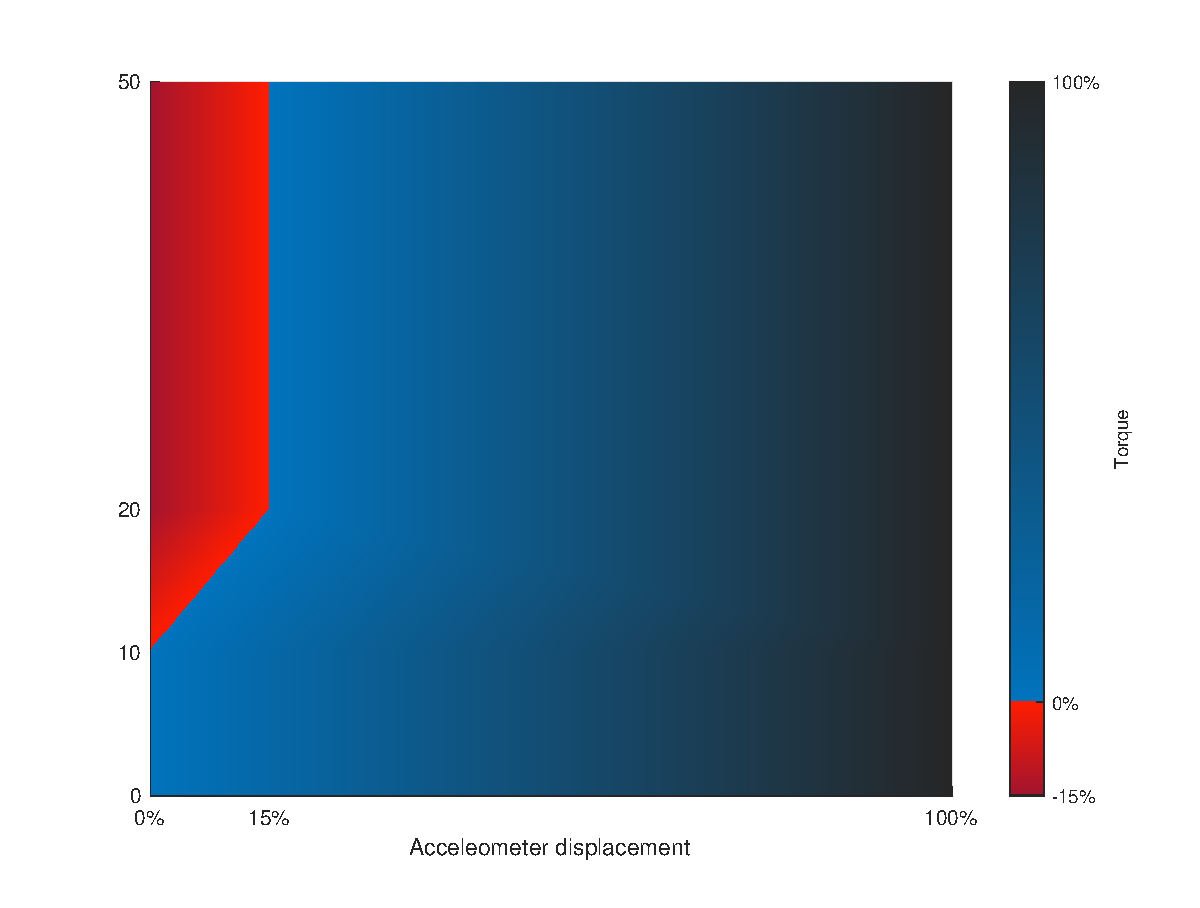
\includegraphics[height=5.8cm]{figures/regen_ideal}
            \label{regen_ideal}
        \caption{Regenerative breaking / torque control}
\end{figure}